\documentclass[tikz,border=2pt]{standalone}
\usepackage{amsmath}
\usepackage{tikz}
\usetikzlibrary{arrows.meta}

\begin{document}
% g∘f: first apply f, then g; the composition is only defined when the outputs of f are
% inputs that g accepts (range of f inside the domain of g).
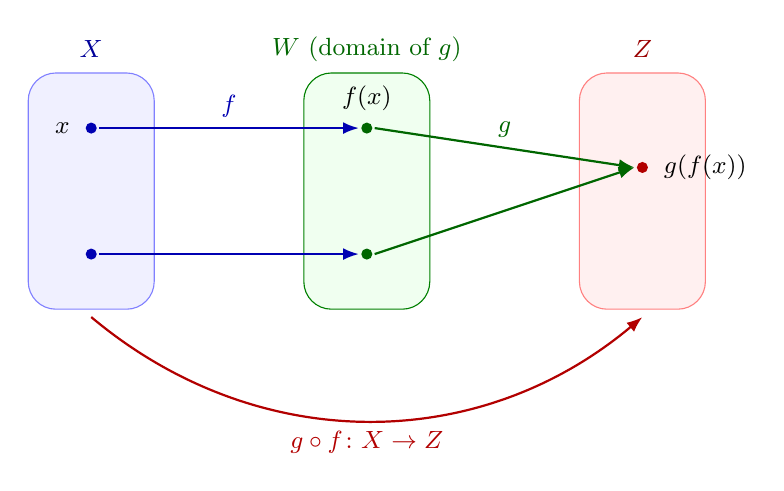
\begin{tikzpicture}[>={Latex[length=2mm]}, every node/.style={font=\small}]
	\draw[rounded corners=10pt, fill=blue!6, draw=blue!50] (-0.8,-1.5) rectangle (0.8,1.5);
	\draw[rounded corners=10pt, fill=green!6, draw=green!50!black] (2.7,-1.5) rectangle (4.3,1.5);
	\draw[rounded corners=10pt, fill=red!6, draw=red!50] (6.2,-1.5) rectangle (7.8,1.5);
	\node[blue!60!black] at (0,1.8) {$X$};
	\node[green!40!black] at (3.5,1.8) {$W$ (domain of $g$)};
	\node[red!60!black] at (7,1.8) {$Z$};
	\foreach \y in {0.8, -0.8} {\fill[blue!70!black] (0,\y) circle (2pt);}
	\foreach \y in {0.8, -0.8} {\fill[green!40!black] (3.5,\y) circle (2pt);}
	\foreach \y in {0.3} {\fill[red!70!black] (7,\y) circle (2pt);}
	\node[left] at (-0.15,0.8) {$x$};
	\node[above] at (3.5,0.9) {$f(x)$};
	\node[right] at (7.15,0.3) {$g(f(x))$};
	\draw[->, blue!70!black, thick] (0.1,0.8) -- node[above] {$f$} (3.4,0.8);
	\draw[->, blue!70!black, thick] (0.1,-0.8) -- (3.4,-0.8);
	\draw[->, green!40!black, thick] (3.6,0.8) -- node[above] {$g$} (6.9,0.3);
	\draw[->, green!40!black, thick] (3.6,-0.8) -- (6.9,0.3);
	\draw[->, thick, red!70!black] (0,-1.6) to[out=-40, in=-140] node[below] {$g\circ f\colon X\to Z$} (7,-1.6);
\end{tikzpicture}
\end{document}
